

%\vspace{-0.1cm}
\section{Experiments}
%\vspace{-0.1cm}

In this section, we evaluate the performances and properties of OCSDF on tabular and image data. All the experiments are conducted with tensorflow, and the 1-Lipschitz neural nets are implemented using the library Deel-Lip\footnote{\url{https://github.com/deel-ai/deel-lip}}. Our code is available at~\url{https://github.com/Algue-Rythme/OneClassMetricLearning}.
%\vspace{-0.2cm}
\subsection{Toy examples from Scikit-Learn}
%\vspace{-0.1cm}

We use two-dimensional toy examples from the Scikit-Learn library~\cite{pedregosa2011scikit}. Results are shown in figure~\ref{fig:toy2d}. The contour of the decision function are plotted in resolution $300\times 300$ pixels. The level sets of the classifier are compared against those of One Class SVM~\cite{scholkopf2001estimating} and Isolation Forest~\cite{liu2008isolation}. We also train a conventional network with Binary Cross Entropy against complementary distribution $Q_t$, and we show it struggles to learn a meaningful decision boundary. Moreover, its Local Lipschitz Constant~\cite{jordan2020exactly} increases uncontrollably, as shown in table~\ref{tab:llc_main}, which makes it prone to adversarial attacks. Finally, there is no natural interpretation of the prediction of the conventional network in terms of distance: the magnitude $|f(\cdot)|$ of the predictions quickly grows above $10^3$, whereas for 1-Lipschitz neural nets, it is approximately equal to the signed distance function $\Sdf$. We refer to Appendix \ref{app:toy2d} for visualizations.


\begin{figure}[!ht]
    \centering
    
    \begin{subfigure}{0.02\linewidth}
    \rotatebox{90}{\small \textbf{OCSDF}} 
    \end{subfigure}
    \begin{subfigure}{0.28\linewidth}
        \centering
        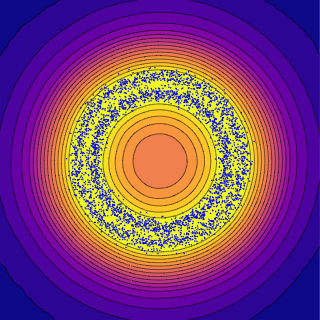
\includegraphics[width=1.\linewidth]{images/ocml/circles_cropped.png}
    \end{subfigure}
    \begin{subfigure}{0.28\linewidth}
        \centering
        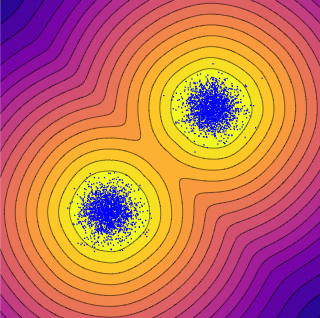
\includegraphics[width=1.\linewidth]{images/ocml/two_blobs_cropped.png}
    \end{subfigure}
    \begin{subfigure}{0.28\linewidth}
        \centering
        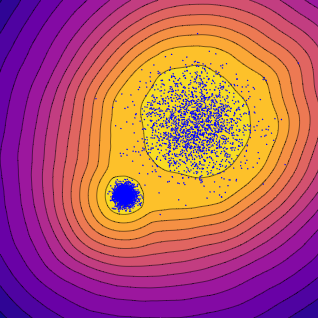
\includegraphics[width=1.\linewidth]{images/ocml/two-blobs-unbalanced_cropped.png}
    \end{subfigure}\\
        \begin{subfigure}{0.02\linewidth}
    \rotatebox{90}{\small \textbf{OCSVM}} 
    \end{subfigure}
    \begin{subfigure}{0.28\linewidth}
        \centering
        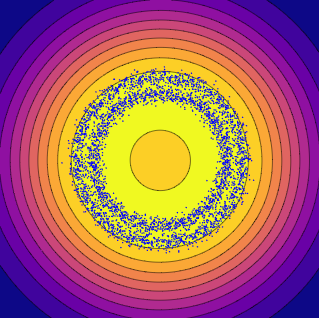
\includegraphics[width=1.\linewidth]{images/ocsvm/ocsvm_circles_cropped.png}
        \subcaption{Two circles.}
    \end{subfigure}
    \begin{subfigure}{0.28\linewidth}
        \centering
        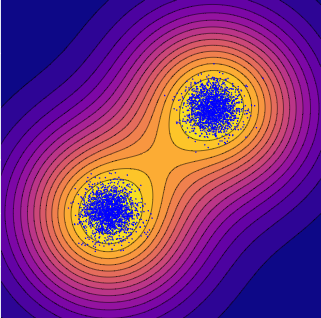
\includegraphics[width=1.\linewidth]{images/ocsvm/ocsvm_two_blobs_cropped.png}
        \subcaption{Two blobs.}
    \end{subfigure}
    \begin{subfigure}{0.28\linewidth}
        \centering
        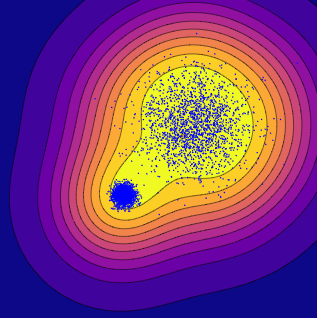
\includegraphics[width=1.\linewidth]{images/ocsvm/ocsvm_two-blobs-unbalanced_cropped.png}
        \subcaption{Blob \& cloud.}
    \end{subfigure}
    \caption{Contour plots of our method with 1-Lipschitz (LIP) network and $\hkr$ (HKR) loss on toy examples of Scikit-learn.}\label{fig:toy2d}
    %\vspace{-0.5cm}
    %Datasets: (a) One blob (b) Two circles (c) Two blobs (d) Two unbalanced blobs (e) Two moons.
\end{figure}

%\vspace{-0.1cm}
\subsection{Anomaly Detection on Tabular datasets}

We tested our algorithm on some of the most prominent anomaly detection benchmarks of ODDS library~\cite{Rayana:2016}. In this unsupervised setting (like ADBench~\cite{han_adbench_nodate}) all the examples (normal examples and anomalies) are seen during training, but their true label is unknown. To apply our method, the only hyperparameter needed is the margin $m$ that we select in the range $[0.01, 0.05, 0.2, 1.]$. For each value, the results are averaged over $20$ independent runs train/test splits. Following ADBench guidelines and best practices from the AD community, we only compute the AUROC, since this metric is symmetric under label flip. We report the best average in table~\ref{tab:tabularrocad} along baselines from ADBench~\cite{han_adbench_nodate}. As observed by~\cite{han_adbench_nodate}, none of the algorithms clearly dominates the others, because what is considered an anomaly (or not) depends on the context. Among 14 other methods tested, our algorithm ranks $7.1 \pm 3.6 / 15$, while the best (Isolation Forests) ranks $4.5 \pm 3.2 / 15$. The experiment shows that our algorithm is competitive with respect to other broadly used baselines. Nonetheless, it brings several additional advantages. First, our algorithm can be seen as a parametric version of kNN for the euclidean distance, which leverages deep learning to avoid the costly construction of structures like a KDTree~\cite{maneewongvatana1999analysis} and the quadratic cost of nearest neighbor search, thereby enabling its application in high dimensions. Second, it provides robustness certificates. We illustrate those two advantages more thoroughly in the next section.


%\vspace{-0.1cm}
\begin{table}[!ht]
    \small
    \centering
    \resizebox{\linewidth}{!}{\begin{tabular}{|c|ccccc|}
        \hline
       \multirow{2}{*}{\makecell{Local Lipschitz\\ Constant}} & \makecell{One\\ Cloud}  & \makecell{Two\\ Clouds} & \makecell{Two\\ Blobs} & \makecell{Blob\\ Cloud} & \makecell{Two\\ Moons} \\
       \cline{2-6}
       &   26.66    &    122.84   &  1421.41  &      53.90     &   258.73  \\ 
       \hline
    \end{tabular}}
    \caption{Lower bound on the Local Lipschitz Constant (LLC) of conventional network after $10,000$ training steps for each toy example. It is the maximum of $\|\nabla_{x_i}f(x_i)\|$ over the train set.}
    \label{tab:llc_main}
    %\vspace{-0.2cm}
\end{table}
\begin{table*}%[]
    \centering
    \small
    %\hspace{-0.35cm}
    \resizebox{\textwidth}{!}{\begin{tabular}{cccc|ccccccc}
    \hline
      Dataset & $\bm{d}$ &\#no.+an. & perc. & \makecell{OCSDF\\ (Ours)} & \makecell{Deep\\ SVDD} & \makecell{OC\\ SVM} & IF & PCA & kNN & SOTA\\
    \hline
    \hline
    % Arrhythmia & 274 & 386+66 & $14.6\%$ & $77.2\pm 0.7$ & N/A & N/A & N/A & N/A & N/A & $81.7$ (ICL)\\
    \multicolumn{4}{c}{Average Rank} & $7.1\pm 3.6$ & $11.2$ & $7.5$ & $4.5$ &  $5.7$ & $7.8$ & $4.5\pm 3.2$ (IF)\\
    \hline  
    breastw & 9 & 444+239 & $35\%$ & $(\#10)\Hquad 82.6\pm 5.9$ & $65.7$ & $80.3$ & $98.3$ & $95.1$ & $97.0$ & $99.7$ (COPOD) \\ 
    cardio & 21 & 1,655+176 & $9.6\%$ & $(\#2)\Hquad 95.0\pm 0.1$ & $59.0$ & $93.9$ & $93.2$ & $95.5$ & $76.6$ & $95.5$ (PCA)\\
    glass & 9 & 205+9 & $4.2\%$ & $(\#7)\Hquad 73.9\pm 4.1$ & $47.5$ & $35.4$ & $77.1$ & $66.3$ & $82.3$ & $82.9$ (CBLOF)\\
    http (KDDCup99) & 3 & 565,287+2,211 & $0.4\%$ & $(\#11)\Hquad 67.5\pm 37$ & $69.0$ & $99.6$ & $99.96$ & $99.7$ & $03.4$ & $99.96$ (IF) \\
    Ionosphere & 33 & 225+126 & $36\%$ & $(\#7)\Hquad 80.2\pm 0.1$ & $50.9$ & $75.9$ & $84.5$ & $79.2$ & $88.3$ & $90.7$ (CBLOF)\\
    Lymphography & 18 & 142+6 & $4.1\%$ & $(\#8)\Hquad 96.1\pm 4.9$ & $32.3$ & $99.5$ & $99.8$ & $99.8$ & $55.9$ & $99.8$ (CBLOF)\\ 
    mammography & 6 & 10,923+260 & $2.32\%$ & $(\#6)\Hquad 86.0\pm 2.5$ & $57.0$ & $84.9$ & $86.4$ & $88.7$ & $84.5$ & $90.7$ (ECOD)\\
    musk & 166 & 2,965+97 & $3.2\%$ & $(\#8)\Hquad 92.6\pm 20.$ & $43.4$ & $80.6$ & $99.99$ & $100.0$ & $69.9$ & $100.0$ (PCA) \\
    Optdigits & 64 & 5,066+150 & $3\%$ & $(\#12)\Hquad 51.0\pm 0.9$ & $38.9$ & $54.0$ & $70.9$ & $51.7$ & $41.7$ & $87.5$ (CBLOF) \\ 
    Pima & 8 & 500+268 & $35\%$ & $(\#12)\Hquad 60.7\pm 1.0$ & $51.0$ & $66.9$ & $72.9$ & $70.8$ & $73.4$ & $73.4$ (kNN) \\
    satimage-2 & 36 & 5,732+71 & $1.2\%$ & $(\#3)\Hquad 97.9\pm 0.4$ & $53.1$ & $97.3$& $99.2$ & $97.6$ & $92.6$ & $99.8$ (CBLOF)\\
    Shuttle & 9 & 45,586+3,511 & $7\%$ & $(\#4)\Hquad 99.1\pm 0.3$ & $52.1$ & $97.4$ & $99.6$ & $98.6$ & $69.6$ & $99.6$ (IF) \\ 
    smtp (KDDCup99) & 3 & 95,126+30 & $0.03\%$ & $(\#4)\Hquad 87.1\pm 3.5$ & $78.2$ & $80.7$ & $89.7$ & $88.4$ & $89.6$ & $89.7$ (IF) \\
    speech & 400 & 3,625+61 & $1.65\%$ & $(\#15)\Hquad 46.0\pm 0.2$ & $53.4$ & $50.2$ & $50.7$ & $50.8$ & $51.0$ & $56.0$ (COF)\\
    thyroid & 6 & 3,679+93 & $2.5\%$ & $(\#5)\Hquad 95.9\pm 0.0$ & $49.6$ & $87.9$ & $98.3$ & $96.3$ & $95.9$ & $98.3$ (IF)\\
    vertebral & 6 & 210+30 & $12.5\%$ &$(\#4)\Hquad 48.6\pm 2.6$ & $36.7$ & $38.0$ & $36.7$ & $37.0$ & $33.8$ & $53.2$ (DAGMM)\\
    vowels & 12 & 1,406+50 & $3.4\%$ & $(\#2)\Hquad 94.7\pm 0.7$ & $52.5$ & $61.6$ & $73.9$ & $65.3$ & $97.3$ & $97.3$ (kNN)\\
    WBC & 30 & 357+21 & $5.6\%$ & $(\#10)\Hquad 93.6\pm 0.1$ & $55.5$ & $99.0$ & $99.0$ & $98.2$ & $90.6$ & $99.5$ (CBLOF) \\ 
    Wine & 13 & 119+10 & $7.7\%$ & $(\#5)\Hquad 81.5\pm 0.9$ & $59.5$ & $73.1$ & $80.4$ & $84.4$ & $45.0$ & $91.4$ (HBOS) \\ 
    %\hline
    \end{tabular}}
    \caption{AUROC score for tabular data, averaged over $20$ runs. The dimension of the dataset is denoted by $\bm{d}$. In the \textbf{Anomaly Detection protocol (AD)} we use all the data (normal class and anomalies) for training, in an unsupervised fashion. The ``\#no.+an.'' column indicates part of normal (no.) and anomalous (an.) data used during training for each protocol. SOTA denominates the best score ever reported on the dataset, obtained by crawling relevant literature, or ADBench~\cite{han_adbench_nodate} results (table D4 page 37). We report the rank as (\#rank) among 14 other methods.\\
    }
    \label{tab:tabularrocad}
    % arrhythmia: ANOMALY DETECTION FOR TABULAR DATA WITH INTERNAL CONTRASTIVE LEARNING (no name => chose ICL)~\cite{shenkar2022anomaly}
    %\footnote{Misleading average: half of the runs yield same AUROC as kNN, and the other half around 99\% AUROC.}
\end{table*}

\begin{table*}%[]
    \centering
    %\hspace{-0.35cm}
    \small
    \resizebox{\textwidth}{!}{\begin{tabular}{c|ccccc|ccc}
    \hline
      MNIST & \makecell{OCSDF} & OCSDF & OCSDF & OCSDF & OCSDF & \makecell{OC\\ SVM} & \makecell{Deep\\ SVDD} & IF \\
      Certificates & $\epsilon=0$ & $\epsilon=8/255$ & $\epsilon=16/255$ & $\epsilon=36/255$ & $\epsilon=72/255$ & $\epsilon=0$ & $\epsilon=0$ & $\epsilon=0$\\
    \hline
    %\hline
    mAUROC &  $\bf 95.5\pm 0.4$ & $93.2\pm 2.1$ & $89.9\pm 3.5$ & $78.4\pm 6.4$ & $57.5\pm 7.5$ & $91.3\pm 0.0$ & $\bf 94.8\pm 0.9$ & $92.3\pm 0.5$\\
    \hline
    digit 0 & $\bf 99.7\pm 0.1$ & $99.6\pm 0.2$ & $99.5\pm 0.2$ & $99.0\pm 0.6$ & $96.2\pm 3.0$ & $98.6\pm 0.0$ & $98.0\pm 0.7$ & $98.0\pm 0.3$\\
    digit 1 & $\bf 99.8\pm 0.0$ & $99.7\pm 0.0$ & $99.6\pm 0.1$ & $99.2\pm 0.3$ & $96.2\pm 1.6$ & $99.5\pm 0.0$ & $\bf 99.7\pm 0.1$ & $97.3\pm 0.4$\\
    digit 2 & $\bf 90.6\pm 2.0$ & $85.3\pm 1.9$ & $78.2\pm 2.3$ & $53.1\pm 5.2$ & $14.1\pm 4.6$ & $82.5\pm 0.1$ & $\bf 91.7\pm 0.1$ & $88.6\pm 0.5$\\
    digit 3 & $\bf 93.4\pm 1.2$ & $90.0\pm 1.7$ & $85.0\pm 2.3$ & $66.2\pm 4.6$ & $26.9\pm 5.0$ & $88.1\pm 0.0$ & $91.9\pm 1.5$ & $89.9\pm 0.4$\\
    digit 4 & $\bf 96.5\pm 0.9$ & $95.3\pm 1.2$ & $93.9\pm 1.7$ & $89.4\pm 3.6$ & $76.2\pm 9.8$ & $94.9\pm 0.0$ & $\bf 94.9\pm 0.8$ & $92.7\pm 0.6$\\
    digit 5 & $\bf 93.9\pm 2.2$ & $89.0\pm 3.2$ & $81.6\pm 4.7$ & $54.0\pm 8.7$ & $15.6\pm 6.9$ & $77.1\pm 0.0$ & $88.5\pm 0.9$ & $85.5\pm 0.8$\\
    digit 6 & $\bf 98.7\pm 0.6$ & $98.1\pm 0.7$ & $97.2\pm 0.9$ & $93.1\pm 2.6$ & $74.9\pm 10.4$ & $96.5\pm 0.0$ & $\bf 98.3\pm 0.5$ & $95.6\pm 0.3$\\
    digit 7 & $\bf 97.1\pm 0.6$ & $96.5\pm 0.5$ & $95.6\pm 0.6$ & $92.2\pm 0.8$ & $81.2\pm 1.7$ & $93.7\pm 0.0$ & $94.6\pm 0.9$ & $92.0\pm 0.4$\\
    digit 8 & $89.4\pm 2.6$ & $83.3\pm 5.1$ & $74.7\pm 9.0$ & $50.3\pm 15.9$ & $24.4\pm 14.0$ & $88.9\pm 0.0$ & $\bf 93.9\pm 1.6$ & $89.9\pm 0.4$\\
    digit 9 & $\bf 96.4\pm 0.3$ & $95.3\pm 0.9$ & $93.8\pm 1.3$ & $87.8\pm 3.1$ & $68.9\pm 7.6$ & $93.1\pm 0.0$ & $\bf 96.5\pm 0.3$ & $93.5\pm 0.3$\\
    %\hline
    \end{tabular}}
    \begin{tabular}{c|ccccc|ccc}
    \hline
      CIFAR10 & \makecell{OCSDF} & OCSDF & OCSDF & OCSDF & OCSDF & \makecell{OC\\ SVM} & \makecell{Deep\\ SVDD} & IF \\
      Certificates & $\epsilon=0$ & $\epsilon=8/255$ & $\epsilon=16/255$ & $\epsilon=36/255$ & $\epsilon=72/255$ & $\epsilon=0$ & $\epsilon=0$ & $\epsilon=0$\\
    \hline
    %\hline
    mAUROC & $57.4\pm 2.1$ & $53.1\pm 2.1$ & $48.8\pm 2.1$ & $38.4\pm 1.9$ & $22.5\pm 1.4$ & $64.8\pm 8.0$ & $64.8\pm 6.8$ & $55.4\pm 8.0$\\
    \hline
    Airplane & $\bf 68.2\pm 4.5$ & $64.3\pm 3.9$ & $60.1\pm 3.2$ & $49.4\pm 1.1$ & $31.2\pm 3.6$ & $61.6\pm 0.9$ & $61.7\pm 4.1$ & $60.1\pm 0.7$\\
    Automobile & $57.3\pm 1.7$ & $52.5\pm 3.0$ & $47.6\pm 4.2$ & $36.1\pm 6.8$ & $19.8\pm 7.8$ & $\bf 63.8\pm 0.6$ & $\bf 65.9\pm 2.1$ & $50.8\pm 0.6$\\
    Bird & $\bf 51.8\pm 2.7$ & $47.5\pm 1.8$ & $43.2\pm 1.6$ & $33.4\pm 3.4$ & $19.5\pm 5.7$ & $\bf 50.0\pm 0.5$ & $\bf 50.8\pm 0.8$ & $\bf 49.2\pm 0.4$\\
    Cat & $\bf 58.8\pm 1.2$ & $54.6\pm 0.8$ & $50.3\pm 0.8$ & $40.0\pm 1.5$ & $24.4\pm 2.3$ & $55.9\pm 1.3$ & $\bf 59.1\pm 1.4$ & $55.1\pm 0.4$\\
    Deer & $49.4\pm 2.4$ & $45.3\pm 2.1$ & $41.4\pm 1.9$ & $32.2\pm 1.5$ & $18.8\pm 1.4$ & $\bf 66.0\pm 0.7$ & $60.9\pm 1.1$ & $49.8\pm 0.4$\\
    Dog & $56.3\pm 0.6$ & $51.9\pm 1.0$ & $47.5\pm 1.6$ & $36.7\pm 2.9$ & $20.6\pm 4.0$ & $62.4\pm 0.8$ & $\bf 65.7\pm 2.5$ & $58.4\pm 0.5$\\
    Frog & $52.6\pm 1.8$ & $48.7\pm 1.7$ & $44.9\pm 1.6$ & $35.8\pm 1.4$ & $22.4\pm 1.1$ & $\bf 74.7\pm 0.3$ & $67.7\pm 2.6$ & $42.9\pm 0.6$\\
    Horse & $49.5\pm 0.9$ & $45.5\pm 1.0$ & $41.5\pm 1.2$ & $32.5\pm 1.5$ & $18.8\pm 1.6$ & $62.6\pm 0.6$ & $\bf 67.3\pm 0.9$ & $55.1\pm 0.7$\\
    Ship & $68.6\pm 1.8$ & $64.6\pm 1.4$ & $60.4\pm 1.3$ & $49.3\pm 2.4$ & $29.8\pm 4.9$ & $\bf 74.9\pm 0.4$ & $\bf 75.9\pm 1.2$ & $\bf 74.2\pm 0.6$\\
    Truck & $61.3\pm 3.4$ & $56.5\pm 2.1$ & $51.5\pm 1.1$ & $39.0\pm 3.9$ & $20.0\pm 7.0$ & $\bf 75.9\pm 0.3$ & $73.1\pm 1.2$ & $58.9\pm 0.7$\\
    %\hline
    \end{tabular}
    \caption{AUROC score on the test set of MNIST and CIFAR10 in a \textit{one versus all} fashion, averaged on $10$ runs. We also report the AUROC of DeepSVDD~\cite{ruff2018deep} for completeness, along with the other AUROC scores of Isolation Forest (IF) and One-Class SVM (OC-SVM) reported in~\cite{ruff2018deep}. When the differences between some
    methods are not statistically significant, we highlight both.  When the confidence intervals overlap, we highlight both. We also show the \textbf{certifiable} AUROC against l-$2$ attacks of norms $\epsilon\in\{8/255,16/255,36/255\}$. Concurrent methods cannot provide certificates for $\epsilon>0$.}
    \label{tab:mnistroc}
\end{table*}



% \begin{table}%[]
%     \centering
%     %\hspace{-0.35cm}
%     \small
%     \begin{tabular}{c|cc}
%     \hline
%       \makecell{Methods\\} & \makecell{CSDFL\\ (ours)} & \makecell{DeepSDF\\ \cite{park2019deepsdf}}\\
%     \hline
%     %\hline
%     Target & \makecell{Generate $Q\bedd P$} & \makecell{Compute $\Sdf(x)$ from $P$}\\
%     Cost         & \makecell{Backward pass} & \makecell{Nearest Neighbor search} \\
%     Loss         & HKR $\hkr$ & $\|f(x)-\Sdf(x)\|^2_2$\\
%     Guarantees   & $f$ is 1-Lipschitz & None\\
%     \end{tabular}
%     \caption{Comparison of our approach against DeepSDF.}
%     \label{tab:comparisondeepsdf}
% \end{table}




%Nonetheless, on F1-score our method beat some significant previous works (see Appendix~\ref{tab:againsthrn}). 

%\vspace{-0.1cm}
\subsection{One Class learning on images}
%\vspace{-0.1cm}

We evaluate the performances of OCSDF for OCC, where only samples of the normal class are supposed to be available. To emulate this setting, we train a classifier on each of the classes of MNIST and Cifar10, and evaluate it on an independent test set in a \textit{one-versus-all} fashion. We compare our method against DeepSVDD \cite{ruff2018deep}, OCSVM \cite{scholkopf_support_1999}, and Isolation Forests \cite{liu2008isolation}. Details on the implementation of the baselines can be found in Appendix \ref{app:occimage}. The mean AUROC score is reported in table~\ref{tab:mnistroc} and averaged over $20$ runs. It is computed between the $1,000$ test examples of the target class and the remaining $9,000$ examples from other classes of the test set (both unseen during training). The histograms of normality scores are given in Appendix \ref{app:occimage}. OCSDF is competitive with respect to other baselines. In addition, it comes with several advantages described in the following. 


%Note that the \textit{out-of-distribution} examples are not seen during training, but more importantly, the \textit{in-distribution} examples from the test set are not seen either. Hence the task evaluates both the generalization capacity (new example from the \textit{in-distribution}) and the discriminative capacity (against \textit{out-of-distribution}). This setting is more challenging because of the curse of dimensionality. 

%Since the models were not available we had to retrain them from scratch. Unfortunately there were discrepancies between the training protocol and the architecture described in original's paper~\cite{ruff2018deep} (LeNet), its official Pytorch repository~\footnote{See \url{https://github.com/lukasruff/Deep-SVDD-PyTorch}.} (LeNet + batch normalization), and its Tensorflow re-implementation from PyOD~\cite{zhao2019pyod} (no convolutions and l$2$-activation regularization). Hence, to allow fair comparison, we run all the versions. We compute the average AUROC over 10 runs, and we keep the best of those runs to compute the empirical AUROC against l$2$-PGD attacks, with the same implementation as Foolbox~\cite{rauber2017foolboxnative}.

%\vspace{-0.1cm}
\subsubsection{Certifiable and empirical robustness}
%\vspace{-0.1cm}

% For each class, we compute the certified AUROC score of each digit for $l_2$ attacks of radii $\epsilon\in\{8/255,16/255,36/255\}$.
None of the concurrent methods can provide certificates against $l_2$ attacks: in the work of~\cite{goyal_drocc_2020} the attacks are performed empirically (no certificates) with $l_\infty$ radii. In table~\ref{tab:mnistroc}, we report our certifiable AUROC with various radii $\epsilon\in\{0, 8/25, 16/255, 36/255, 72/255\}$. In figure~\ref{fig:robust} we report the empirical AUROC against $l_2$-PGD attacks with three random restarts, using stepsize $\zeta=0.025\epsilon$ like Foolbox~\cite{rauber2017foolboxnative}. These results illustrate our method's benefits: not only does it come with robustness certificates that are verified empirically, but the empirical robustness is also way better than DeepSVDD, especially for Cifar10. Note that for 1-Lipschitz network trained with $\hkr$ loss, all the attacks tend to find the same adversaries~\cite{serrurier2021achieving} - hence PGD is also representative of the typical score that would have been obtained with other attack methods.


\begin{figure}[!ht]
%\vspace{-0.2cm}
    \centering
    \begin{subfigure}{0.22\textwidth}
        \centering
        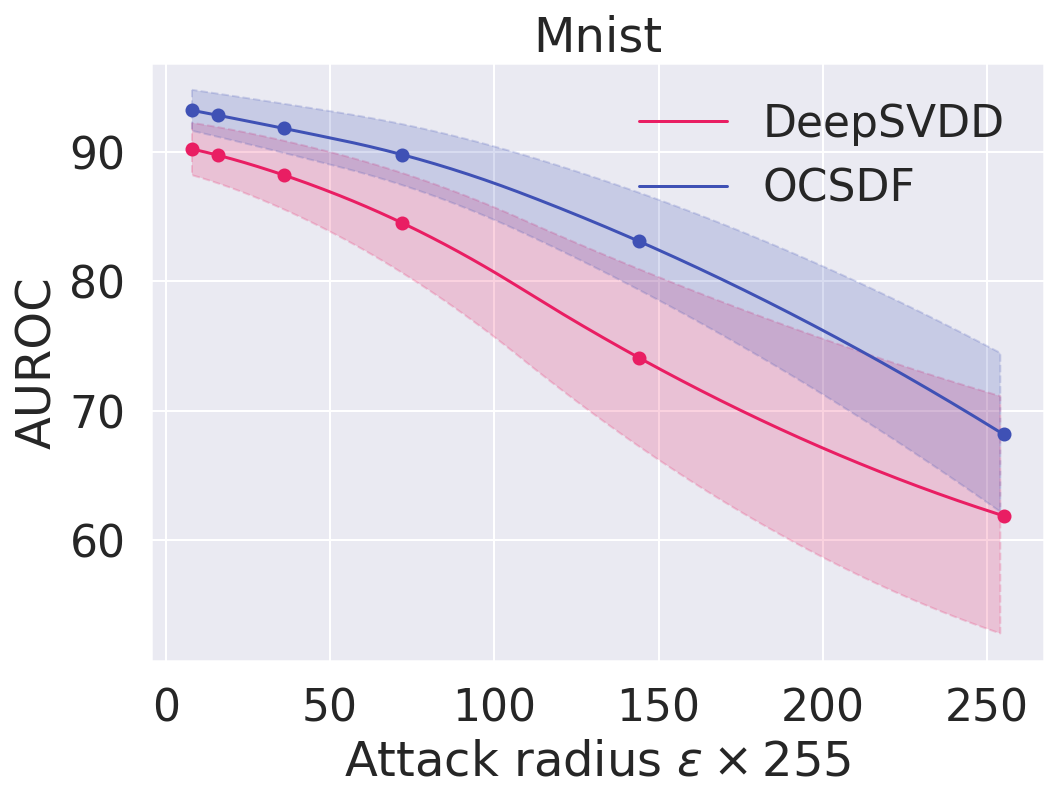
\includegraphics[scale=0.2]{new_images/graphs/mnist_auroc_robust.png}
    \end{subfigure}
    \begin{subfigure}{0.22\textwidth}
        \centering
        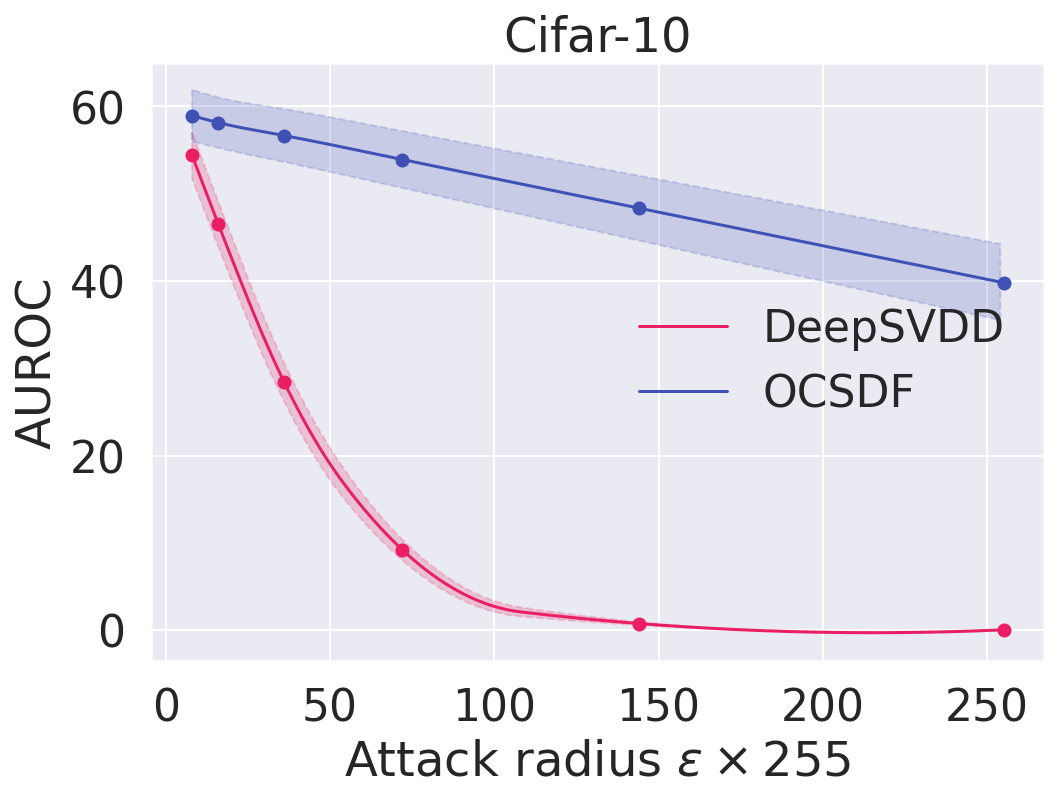
\includegraphics[scale=0.2]{new_images/graphs/cifar_auroc_robust.png}
    \end{subfigure}
    \caption{Empirical Mean AUROC on all classes against adversarial attacks of various radii in One Class setting, using default parameters of FoolBox~\cite{rauber2017foolboxnative}.}
    %\vspace{-0.15cm}
    \label{fig:robust}
\end{figure}
%Note that the certificates are generally pessimistic, and Eikhonal equation gap $1-\|\nabla_x f(x)\|_2^2$ translates into larger difference between certificates and empirical robustness.


%\vspace{-0.1cm}
\subsubsection{Visualization of the support}
%\vspace{-0.1cm}


OCSDF can be seen as a parametric version of kNN, which enables this approach in high dimensions. As a result, the decision boundary learned by the classifier can be materialized by generating adversarial examples with algorithm~\ref{alg:newtonraphson}. The forward computation graph is a classifier based on optimal transport, and the backward computation graph is an image generator. Indeed, the back-propagation through a convolution is a transposed convolution, a popular layer in the generator of GANs. Overall, the algorithm behaves like a WGAN~\cite{arjovsky2017wasserstein} with a single network fulfilling both roles. This unexpected feature opens a path to the explainability of the One Class classifier: the support learned can be visualized without complex feature visualization tools. In particular, it helps identify failure modes.
 
 %\vspace{-0.1cm}
 \begin{figure}[!ht]
    \centering
    
    %% 0 1
    \begin{subfigure}{0.24\textwidth}
        \centering
        
\includegraphics[width=1.\textwidth]{new_images/mnist/gan_0_cropped.PNG}
    \end{subfigure}\begin{subfigure}{0.24\textwidth}
        \centering
        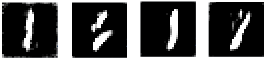
\includegraphics[width=1.\textwidth]{new_images/mnist/gan_1_cropped.png}
    \end{subfigure}
    
    %% 2 3
    \begin{subfigure}{0.24\textwidth}
        \centering
        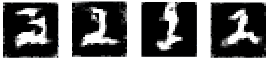
\includegraphics[width=1.\textwidth]{new_images/mnist/gan_2_cropped.png}
    \end{subfigure}\begin{subfigure}{.24\textwidth}
        \centering
        
\includegraphics[width=1.\textwidth]{new_images/mnist/gan_3_cropped.png}
    \end{subfigure}
    
    
    \caption{Examples from algorithm~\ref{alg:newtonraphson} with $T=64$ and $\eta=1$.}\label{fig:mnist_gen_main}
    %\vspace{-0.3cm}
    %Datasets: (a) One blob (b) Two circles (c) Two blobs (d) Two unbalanced blobs (e) Two moons.
\end{figure}


%\vspace{-0.1cm}
\subsubsection{Limitations}
%\vspace{-0.1cm}

We also tested our algorithm on the Cats versus Dogs dataset by training on Cats as the One Class and using Dogs as OOD examples. On this high-dimensional dataset, the AUROC barely exceeds $55.0\%$. This suggests that the SDF is relevant for tabular and simple image datasets (e.g MNIST) but fails to generalize in a meaningful way in higher dimensions. The distance used to define the learned SDF is the euclidian distance. It is well known that such distance has its limitations in pixel space. Using different distances that are more relevant to pixel space is a perspective left for future works.  Our constructions rely on our ability to solve Eikonal equation $\|\nabla_x f\|=1$. This is easy to enforce on dense layers, but it is still an active research area for convolutions (see the recent works of~\cite{achour2021existence,singlaimproved2022,xulot2022}).  

In addition, scores reported in Table~\ref{tab:mnistroc} use the same hyper-parameters for all the classes of Cifar-10, while some concurrent approaches~\cite{goyal_drocc_2020} tune them on a per-class basis. We observed significant improvements with per class tuning of the margin (see figure~\ref{tab:cheatingprotocolcifar} in appendix), but we chose not to report them in Table~\ref{tab:mnistroc}, because this practice is criticized by recent contributions on which we are aligned~\cite{han_adbench_nodate,dinghyperparameter2022}.
%A more thorough discussion of the limitations is left in Appendix~\ref{app:limitations}.





%\vspace{-0.1cm}
\section{OCSDF for implicit shape parametrization}
%\vspace{-0.1cm}
Our approach to learning the SDF contrasts with the computer graphics literature, where SDF is used to obtain the distance of a point to a surface (here defined as $\partial\support$). Indeed, SDFs are usually learned in a supervised fashion, requiring the ground truth of $l_2$ distance. This is classically achieved using Nearest-Neighbor algorithms, which can be cumbersome, especially when the number of points is high. Efficient data structures (e.g., using K-dtrees~\cite{maneewongvatana1999analysis} or Octrees~\cite{meagher1980octree}) can mitigate this effect but do not scale well to high dimensions. Instead, OCSDF learns the SDF solely based on points contained in the support.  While neural network training is not cheap by any mean, the network approach is advantageous at inference time. Indeed, with a dataset of size $n$, a single forward in the network costs $\BigO(1)$ (furthermore orthogonalization of matrices can be done once for all), while kNN costs $\BigO(n^2)$ or $\BigO(n\log{n})$ (with trees).

\begin{figure}[!ht]
    \centering
    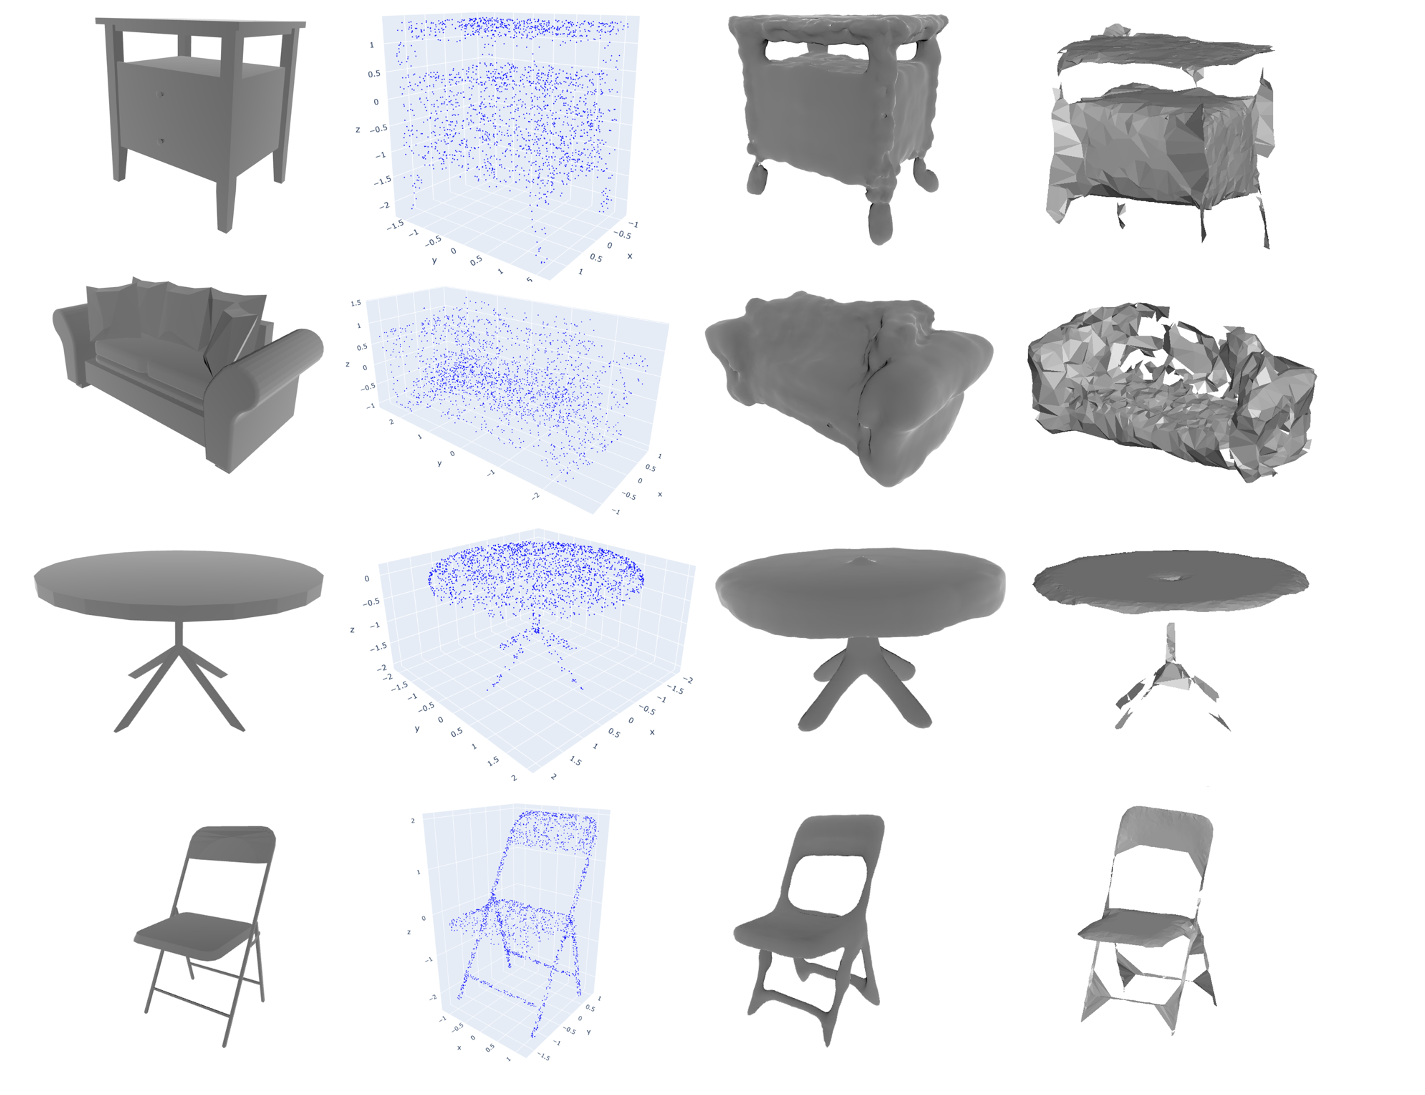
\includegraphics[width=1.\linewidth, trim=0 2.6cm 0 0, clip]{new_images/meshes/reduced_merged.png}
    \caption{Visualization of the SDF (3rd column) from sparse point clouds of size $2048$ (2nd column) sampled from ground truth meshes (1st column) with \textit{Trimesh} library, against the SSSR algorithm~\cite{boltcheva2017surface} that attempts to reproduce the meshes solely from a point cloud (4th column). The SDF exhibits better extrapolation properties and provides smooth surfaces.}
    \label{fig:modelnet3d}
    %\vspace{-0.3cm}
\end{figure}

To illustrate this, we use models from {Princeton's ModelNet10 dataset~\cite{wu20153d}}. We sample $n=2048$ within each mesh to obtain a 3d point cloud. We fit the SDF on the point cloud with the same hyperparameters as the tabular experiment. We use Lewiner marching algorithm~\cite{lewiner2003efficient} from scikit-image~\cite{van2014scikit}, on a $200\times 200\times 200$ voxelization of the input. We plot the mesh reconstructed with Trimesh~\cite{trimesh}. The results are highlighted in figure~\ref{fig:modelnet3d}. We chose the first percentile of $\Expect_{x\sim \Prob_X}[f(x)]$ as the level set of the iso-surface we plot. We compare our results visually against a baseline from~\cite{boltcheva2017surface} implemented in Graphite~\cite{graphite} that rebuilds the mesh solely from the point cloud (without extrapolation). We highlight that $n=2048$ is considered low resolution; hence many details are expected to be lost. Nonetheless, our method recovers the global aspect of the shape more faithfully, smoothly, and consistently than the other baseline. 

%\vspace{-0.1cm}




%In table~\ref{tab:comparisondeepsdf} we highlight some key differences of our approach with the seminal work of~\cite{park2019deepsdf} on SDF in computer graphics. This table emphasizes that our method can be applied more 


